\documentclass{article}
\usepackage[utf8]{inputenc}
\usepackage{graphicx}
\usepackage{float}
\usepackage[a4paper,
            left=1in,
            right=1in,
            top=0.5in,
            bottom=1in,]{geometry}



\title{Is Florida Getting Warmer?}
\author{Kayleigh Greenwood}
\date{November 2021}

\begin{document}

\maketitle

\section{Results}
The Kendall rank correlation coefficient was used to determine whether there was a positive correlation between Year and Temperature in Key West, Florida. The correlation coefficient of the Temperature data throughout the years in the 20th century was 0.371887, and a permutation analysis (Figure 1) of 1000 shuffled populations was used to determine the approximate, asymptotic, one-tailed P-value of 0.

\begin{figure}[H]
\centering
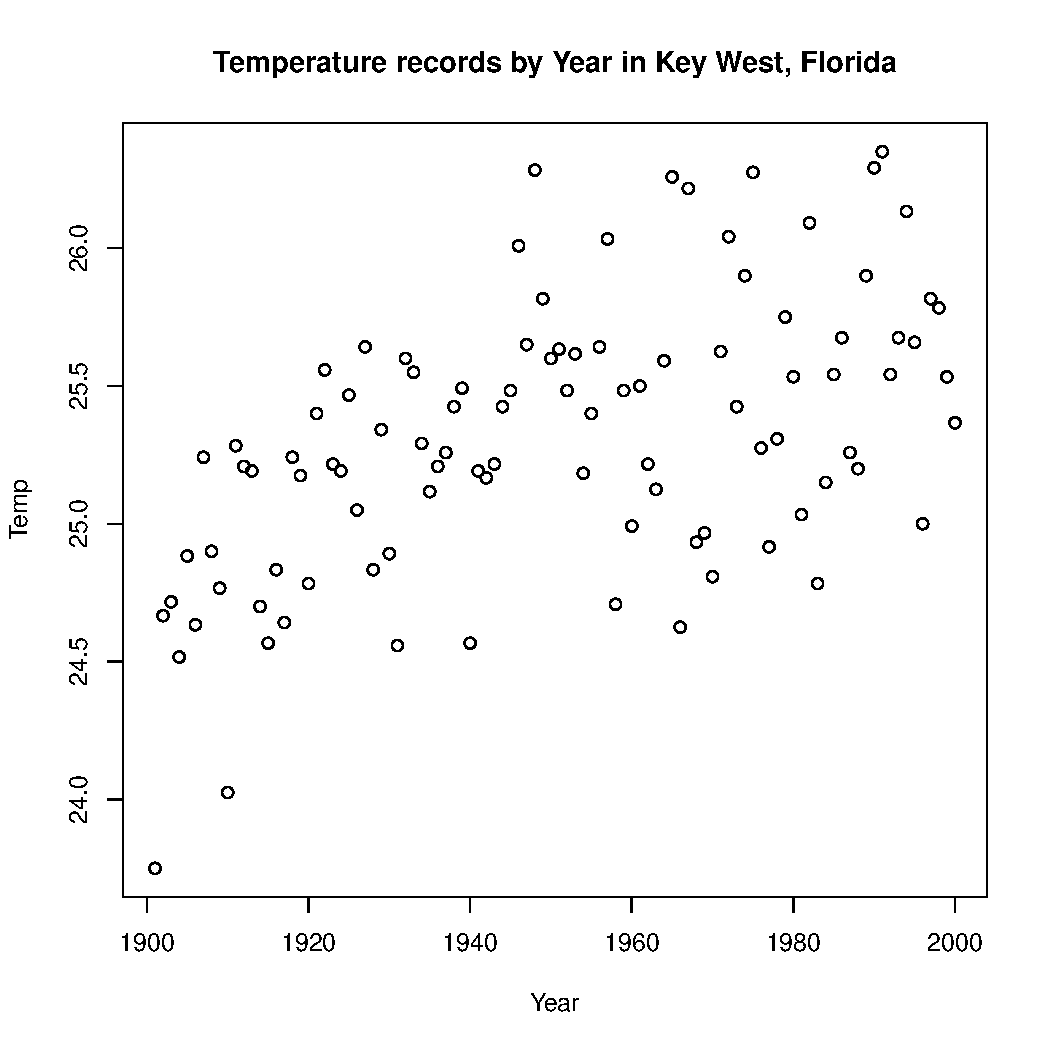
\includegraphics[scale=0.75]{../results/atsplot.pdf}
\caption{Raw data of Temperature over time}
\end{figure}

\begin{figure}[H]
\centering
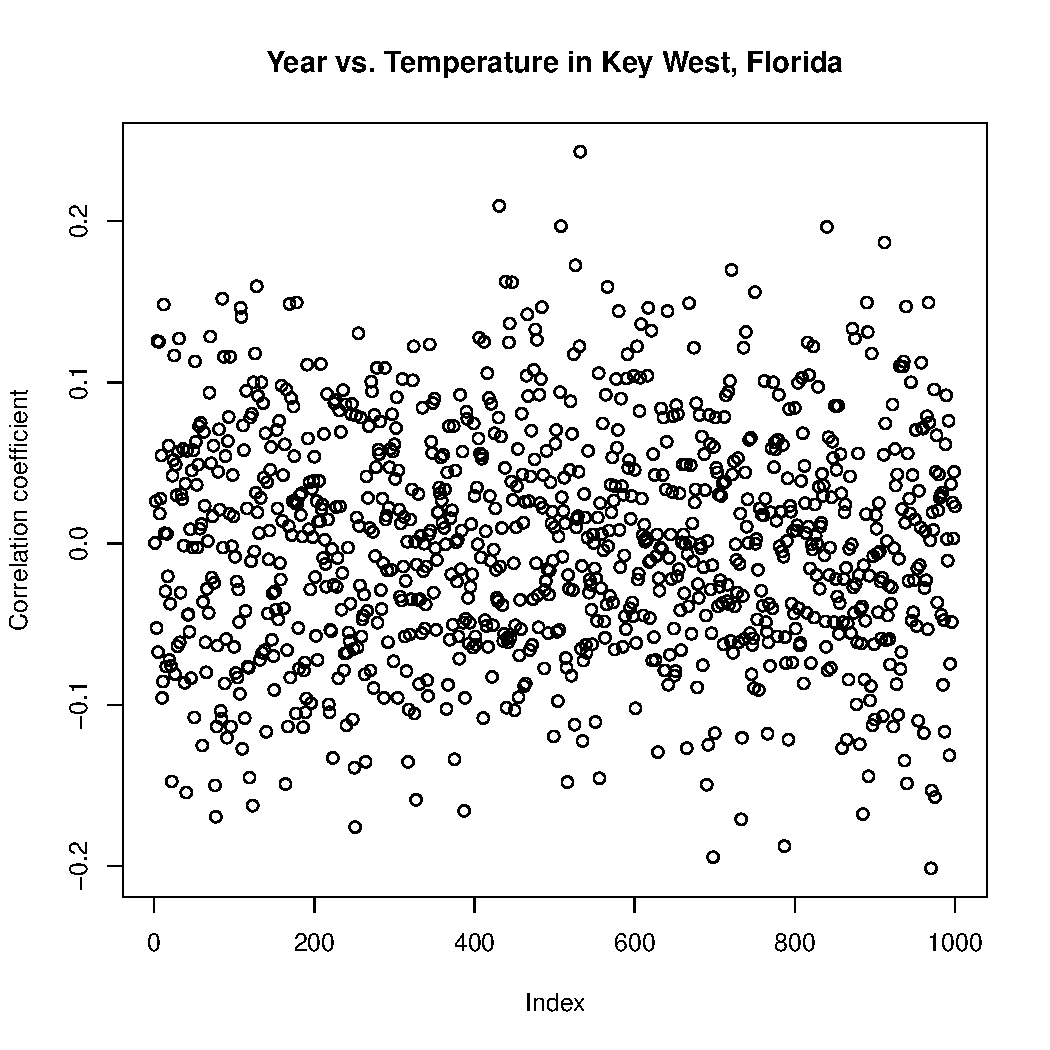
\includegraphics[scale=0.75]{../results/allcoeffs.pdf}
\caption{Coefficients}
\end{figure}

\begin{figure}[H]
\centering
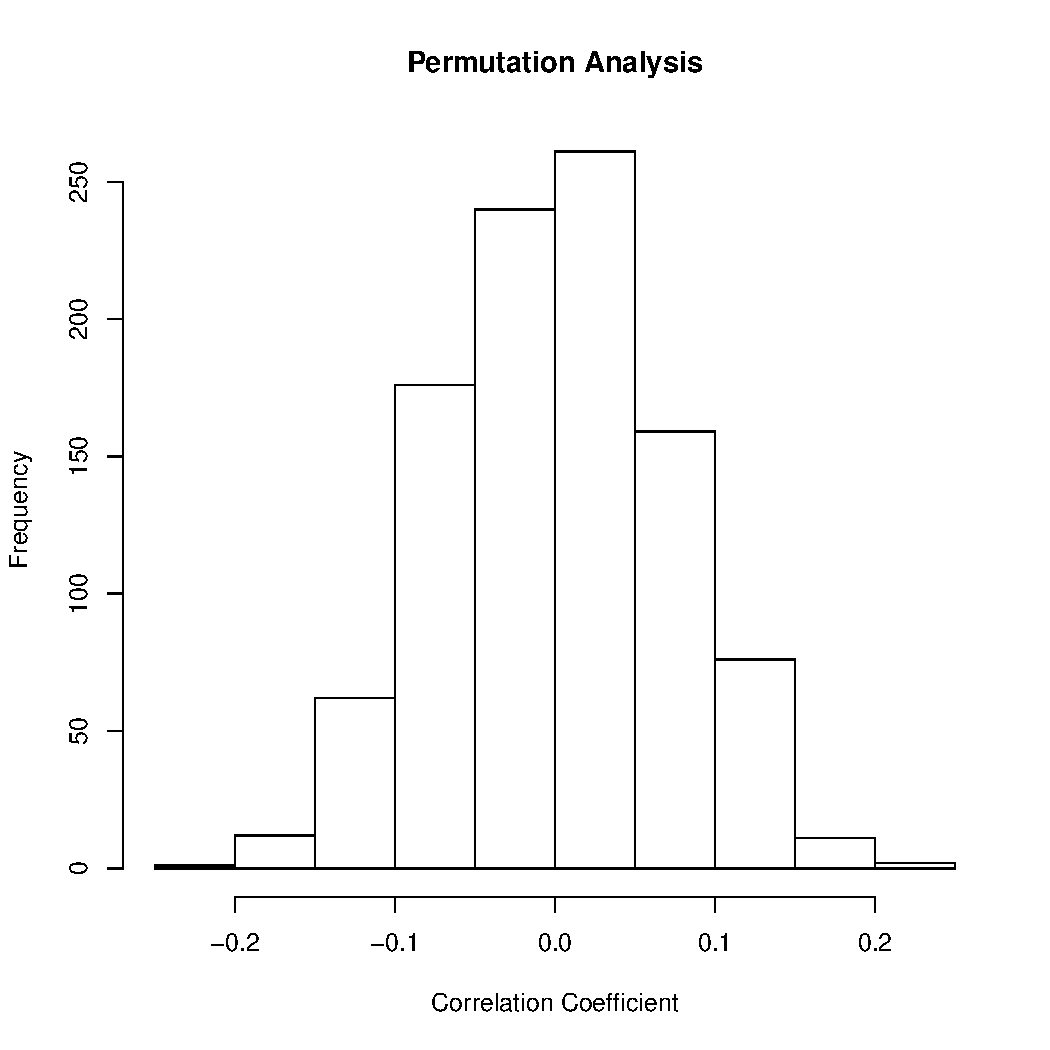
\includegraphics[scale=0.75]{../results/allcoeffshist.pdf}
\caption{Histogram of Coefficients}}
\end{figure}

\section{Discussion}
 Given that the P-value was below 0.05, we can reject the null hypothesis that there is no relationship between Time and Temperature in Key West, Florida, and determine that there is a statistically significant positive correlation between the two variables. The positive correlation indicated between Year and Temperature in Key West is statistically significant.
These results suggest that throughout the 20th century, temperature was increasing over time in Key West.

\end{document}
